\textbf{\large Результаты}

\begin{enumerate}
\item Замеры времени работы ядер с различными конфигурациями (время указано в микросекундах).

\begin{tabular}{|c|c|c|c|c|c|}\hline
\diaghead{\theadfont Diag ColumnmnHead II}%
{Конфи-\\гурации ядра}{Размер изо-\\ бражений}&
\thead{16x16}&\thead{256x256}&\thead{1280x720}&\thead{1920x1080}&\thead{3840x2160}\\
\hline
1, 32 & 13 & 213 & 3186 & 7154 & 28603\\
\hline
32, 32 & 8 & 16 & 150 & 321 & 1263\\
\hline
32, 256 & 8 & 11 & 52 & 97 & 357\\
\hline
256, 256 & 8 & 13 & 50 & 92 & 282\\
\hline
1024, 1024 & 63 & 64 & 107 & 144 & 352\\
\hline
\end{tabular}

\item Сравнение с CPU

\begin{tabular}{|c|c|c|c|c|c|}\hline
Размер входных данных &
\thead{16x16}&\thead{256x256}&\thead{1280x720}&\thead{1920x1080}&\thead{3840x2160}\\
\hline
GPU(256, 256) & 8 & 13 & 50 & 92 & 282\\
\hline
CPU & 1 & 353 & 5126 & 10985 & 43778\\
\hline
\end{tabular}

\item Примеры изображений

%\begin{figure}[htb]
%{
%\centering
\begin{figure}[H]
\begin{minipage}{0.5\textwidth}
  %\centering
  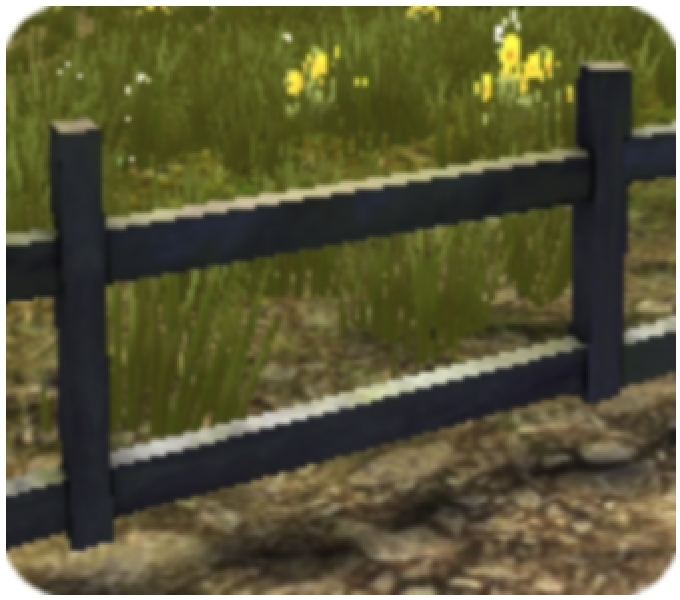
\includegraphics[width=1.0\linewidth]{src/test1.png}
  \captionof{figure}{До SSAA}
  %\label{fig:test1}
\end{minipage}%
\begin{minipage}{0.5\textwidth}
  %\centering
  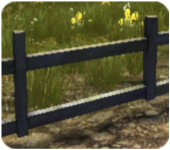
\includegraphics[width=1.0\linewidth]{src/ans1.png}
  \captionof{figure}{После SSAA}
  %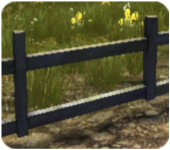
\includegraphics[width=.4\linewidth]{src/ans1.png}
  %\captionof{figure}{Another figure}
  %\label{fig:test2}
\end{minipage}
\end{figure}
%}
%\end{figure}

\begin{figure}[H]
\begin{minipage}{0.5\textwidth}
  %\centering
  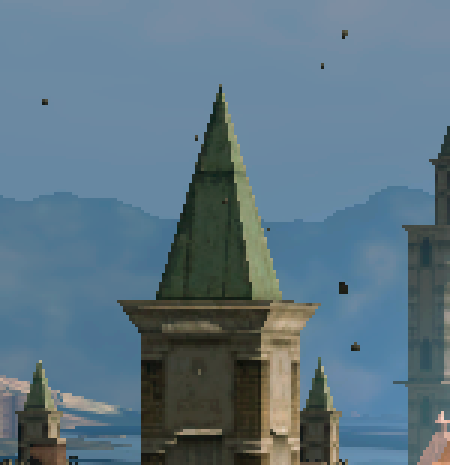
\includegraphics[width=0.95\linewidth]{src/test3.png}
  \captionof{figure}{До SSAA}
  %\label{fig:test1}
\end{minipage}%
\begin{minipage}{0.5\textwidth}
  %\centering
  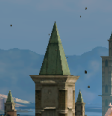
\includegraphics[width=0.95\linewidth]{src/ans3.png}
  \captionof{figure}{После SSAA}
  %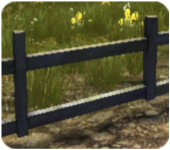
\includegraphics[width=.4\linewidth]{src/ans1.png}
  %\captionof{figure}{Another figure}
  %\label{fig:test2}
\end{minipage}
\end{figure}

\end{enumerate}

